\section{Hardware Components and Construction}

\subsection{Cooling and air purging system}

The SVT regions are cantilevered off a chilled cold plate that is designed to remove the heat generated by the electronics and to provide operational  conditions for the sensors. External cooling has been chosen over internal cooling (tubes in the modules) to keep the amount of material in the active area as low as possible. The front-end electronics provide 5 W per module, with the 42 total modules producing 210 W. The HFCB flex cables are routed through 10 mm slots in the cold plate. The cold plate (see Fig.~\ref{fig:coldplate}) includes a copper plate with brazed  copper 0.25 in inner diameter tubes and a PEEK plate on the upstream side. The sensors are cooled by cold air.  The coolant lines to and from the cold plate are placed inside of 0.5 in diameter nylon tubes.  Air flows inside the 0.5 in tubes, outside the coolant tubes, to cool the air.  The air flows out of the 0.25 in tubes through holes in the cold plate, into the sensor area.

\begin{figure}[hbt] 
\centering 
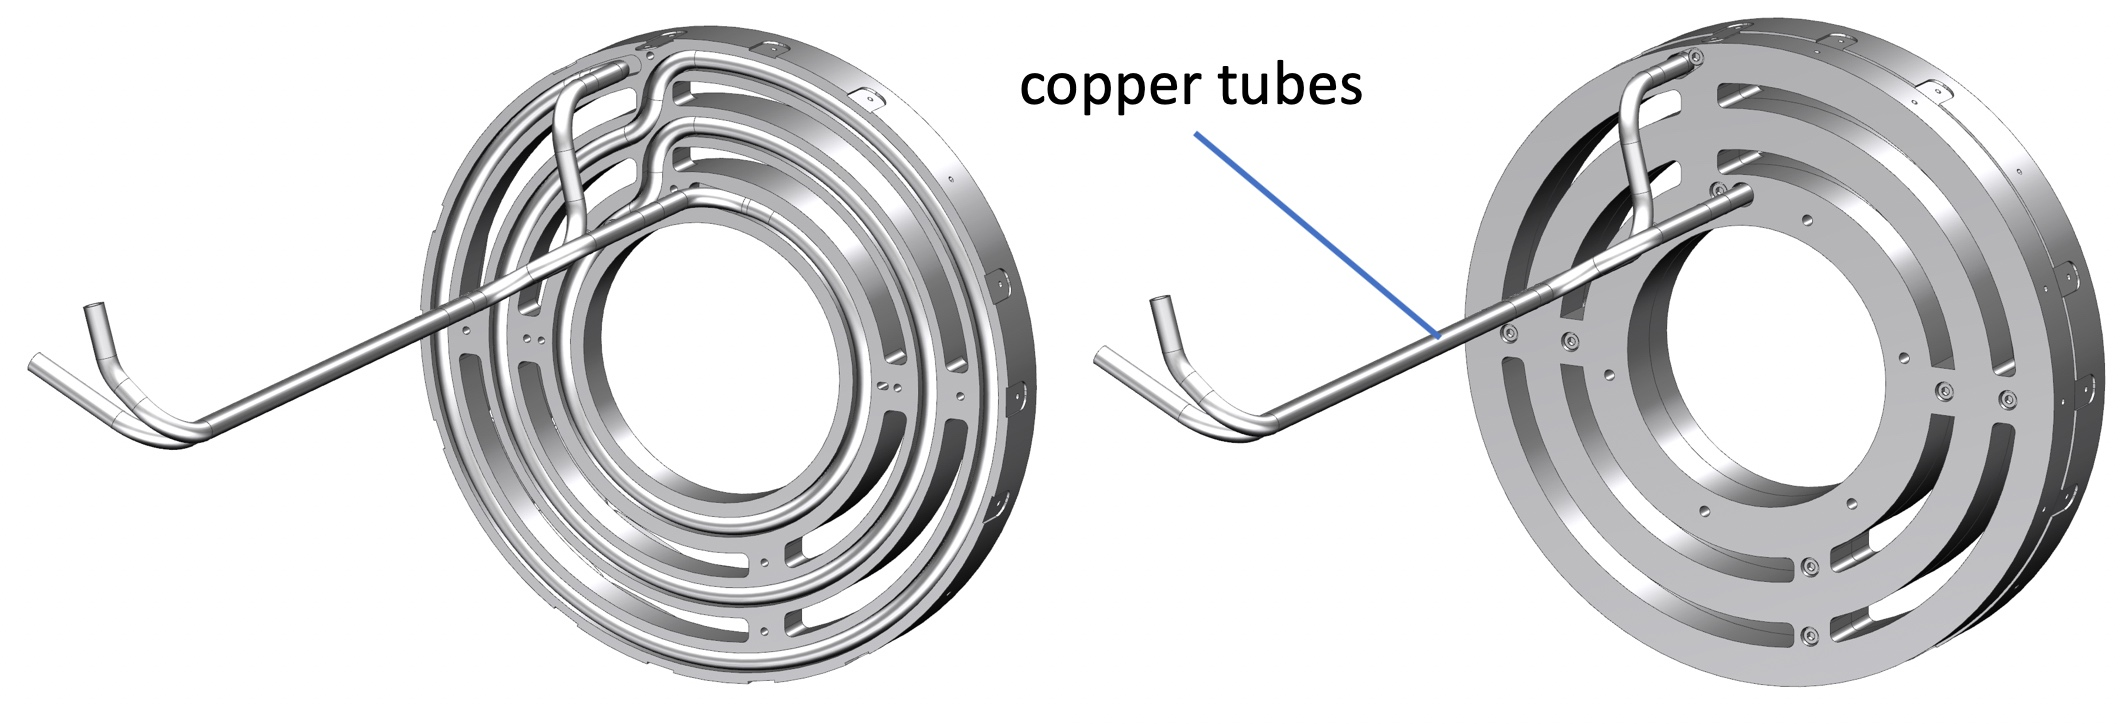
\includegraphics[width=1.0\columnwidth,keepaspectratio]{coldplate.jpg}
\caption{Copper tubing lines brazed to the copper cold plate (left) and the fully assembled assembled cold plate (right).}
\label{fig:coldplate}
\end{figure}

%\begin{wrapfigure}{l}{0.5\columnwidth}
%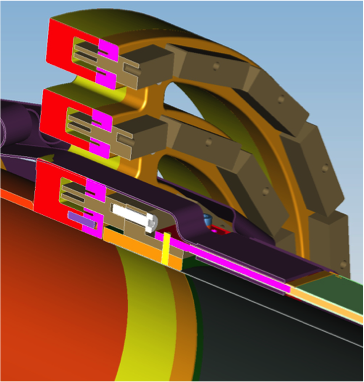
\includegraphics[width=1.0\columnwidth]{cold_plate.png}
%\caption{Routing flex cable through the cold plate.}
%\label{fig:cold-plate}
%\end{wrapfigure}

Coolant (Dynalene HC50) flows at a rate of 2 liters per minute at a temperature of -25$\degree$C. The cold plate upstream cover is made of PEEK plastic. Dry air flowing through the slots in the cold plate is cooled by the liquid coolant circulating in the tube inside the air purging line (see Fig.~\ref{fig:purging1}). With 100 liters per minute of chilled air flow across the cold plate, the sensors are cooled to the operational temperature of -10$\degree$C. The Faraday cage cap on the downstream end has 4 holes to ensure the flow of cold air along the barrel. 

\begin{figure}[hbt] 
\centering 
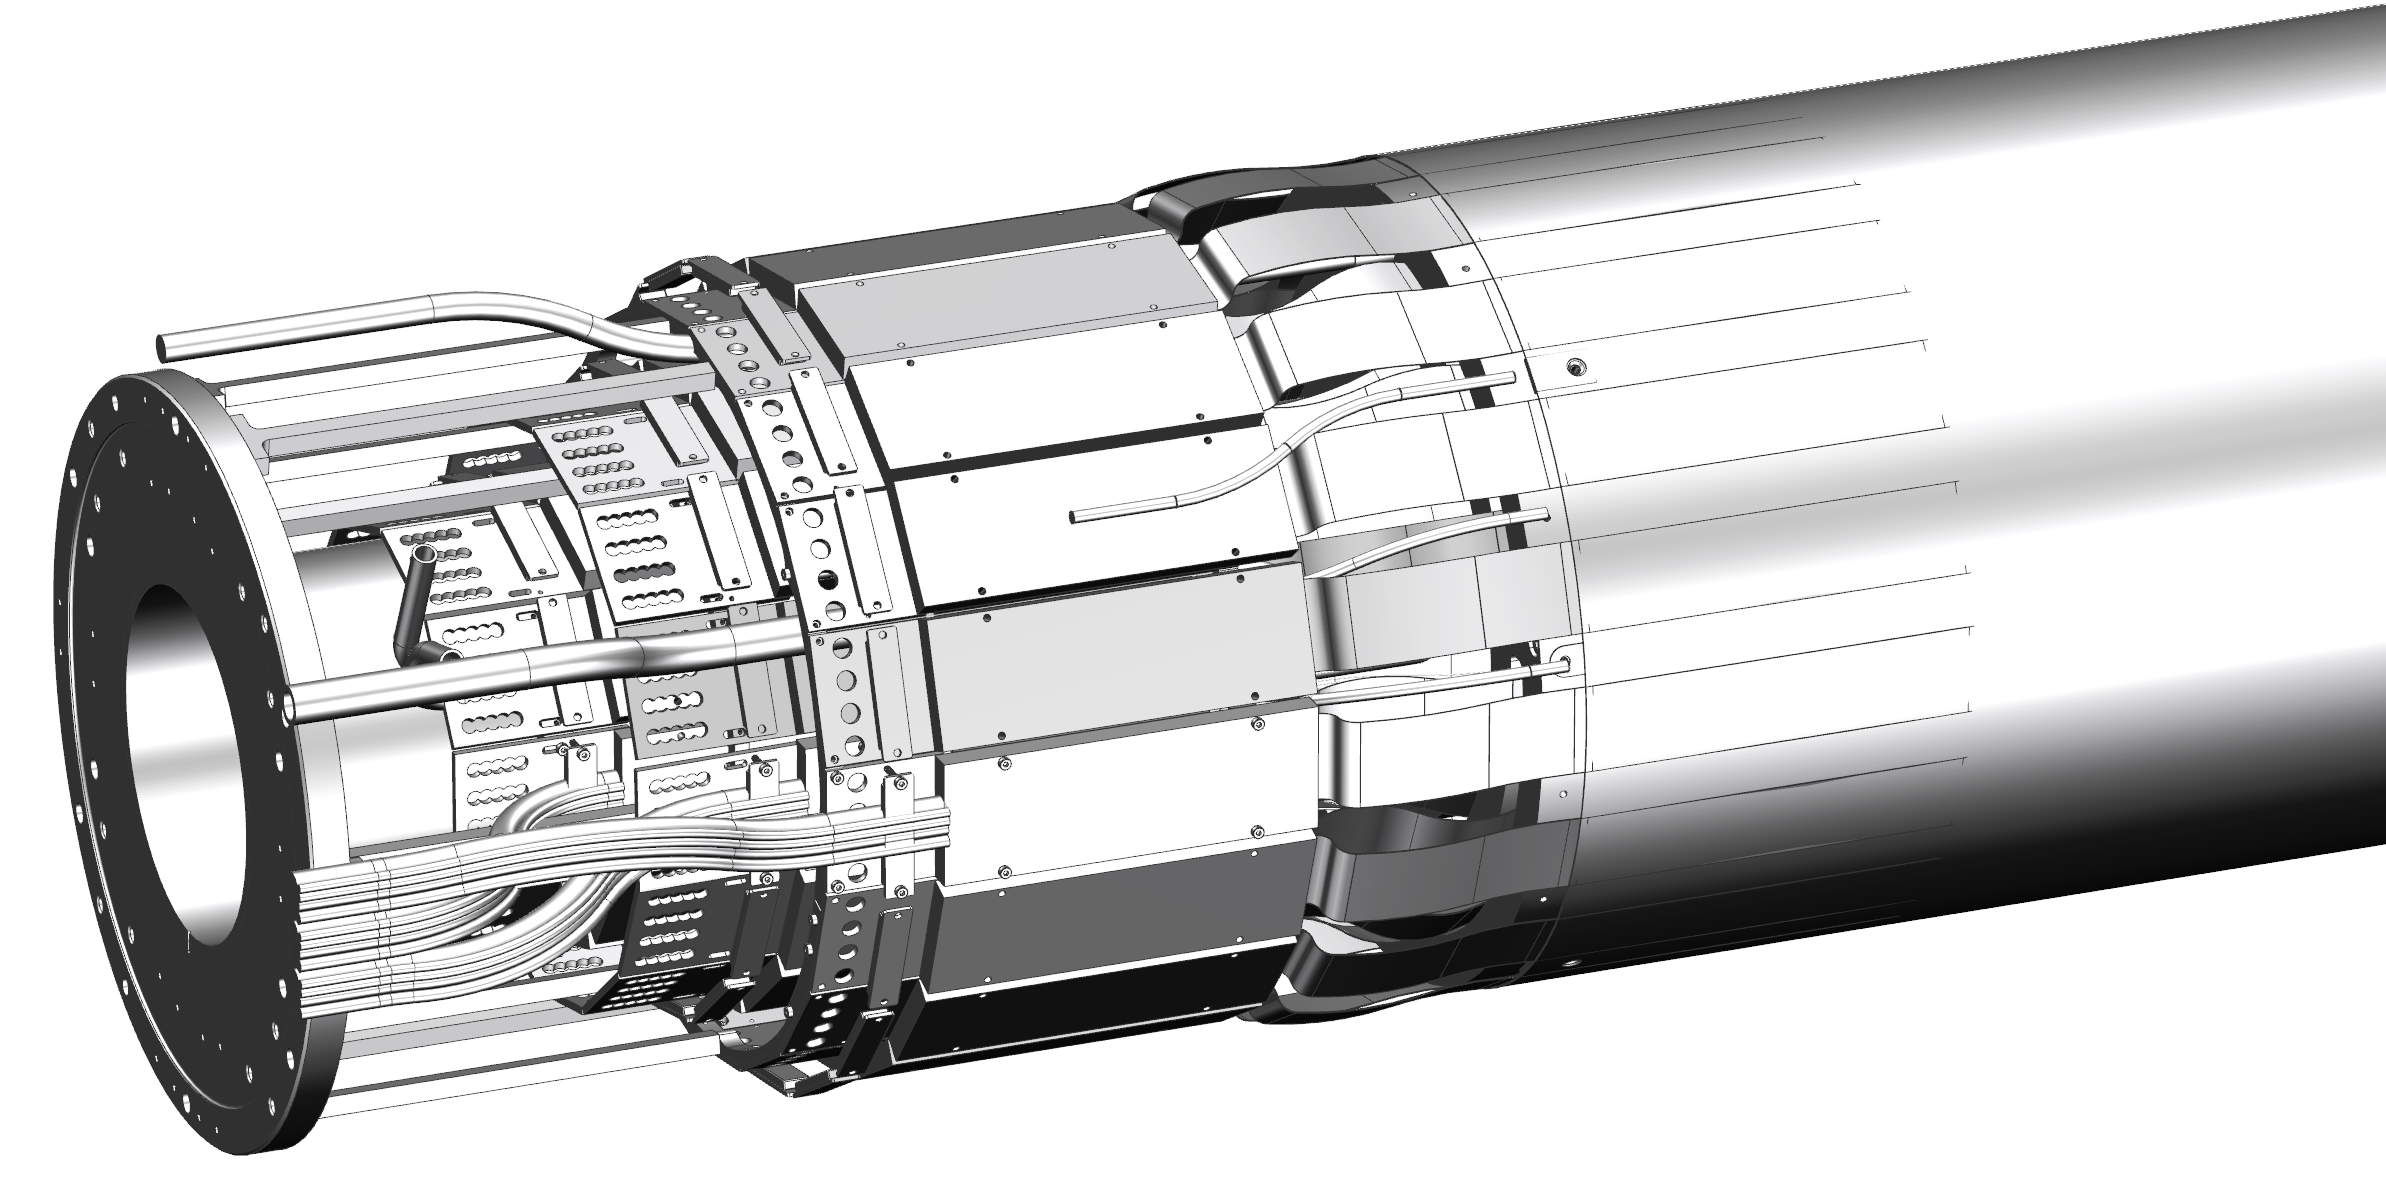
\includegraphics[width=1.0\columnwidth,keepaspectratio]{purging1.png}
\caption{Dry air flows past connectors, through the slots in the cold plate, into the Faraday cage, past sensors, and out through the holes in the cap.}
\label{fig:purging1}
\end{figure}

\begin{figure}[hbt] 
\centering 
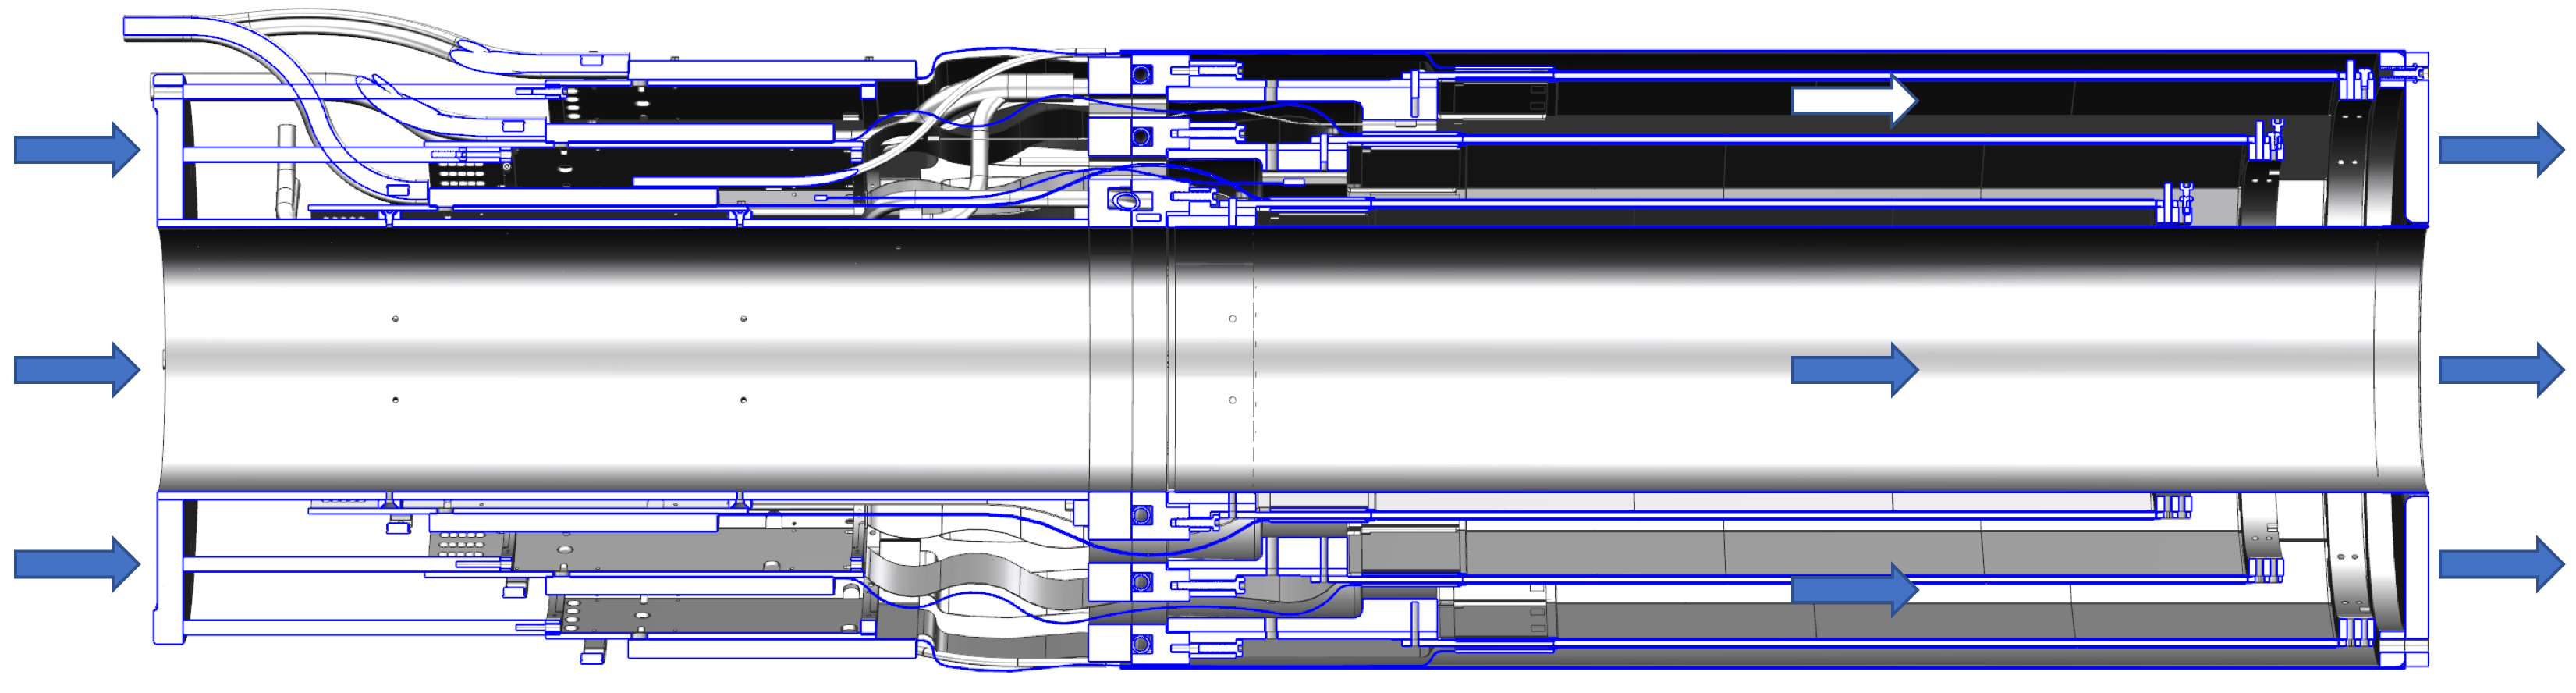
\includegraphics[width=1.0\columnwidth,keepaspectratio]{purging2.png}
\caption{Cross section of the SVT detector showing the dry air flow.}
\label{fig:purging2}
\end{figure}

The outer shell of the Faraday cage is insulated with a 3-mm-thick neoprene sheet. The barrel is protected from environment humidity by purging dry air between the scattering chamber and the inner shell of the Faraday cage and between the outer shell of the Faraday cage and the protective plastic cover (see Fig.~\ref{fig:purging2}). 

\subsection{Slow controls and detector monitoring}

Ambient conditions inside the detector are monitored by temperature and humidity sensors installed on the upstream rings (see Fig.~\ref{fig:ambient-sensors}). There are 3 ambient sensor boards glued in dedicated slots on the inner side of the rings in Regions 2 and 3. There are 2 temperature and 2 humidity sensors on each board for redundancy. 

\begin{figure}[hbt] 
\centering 
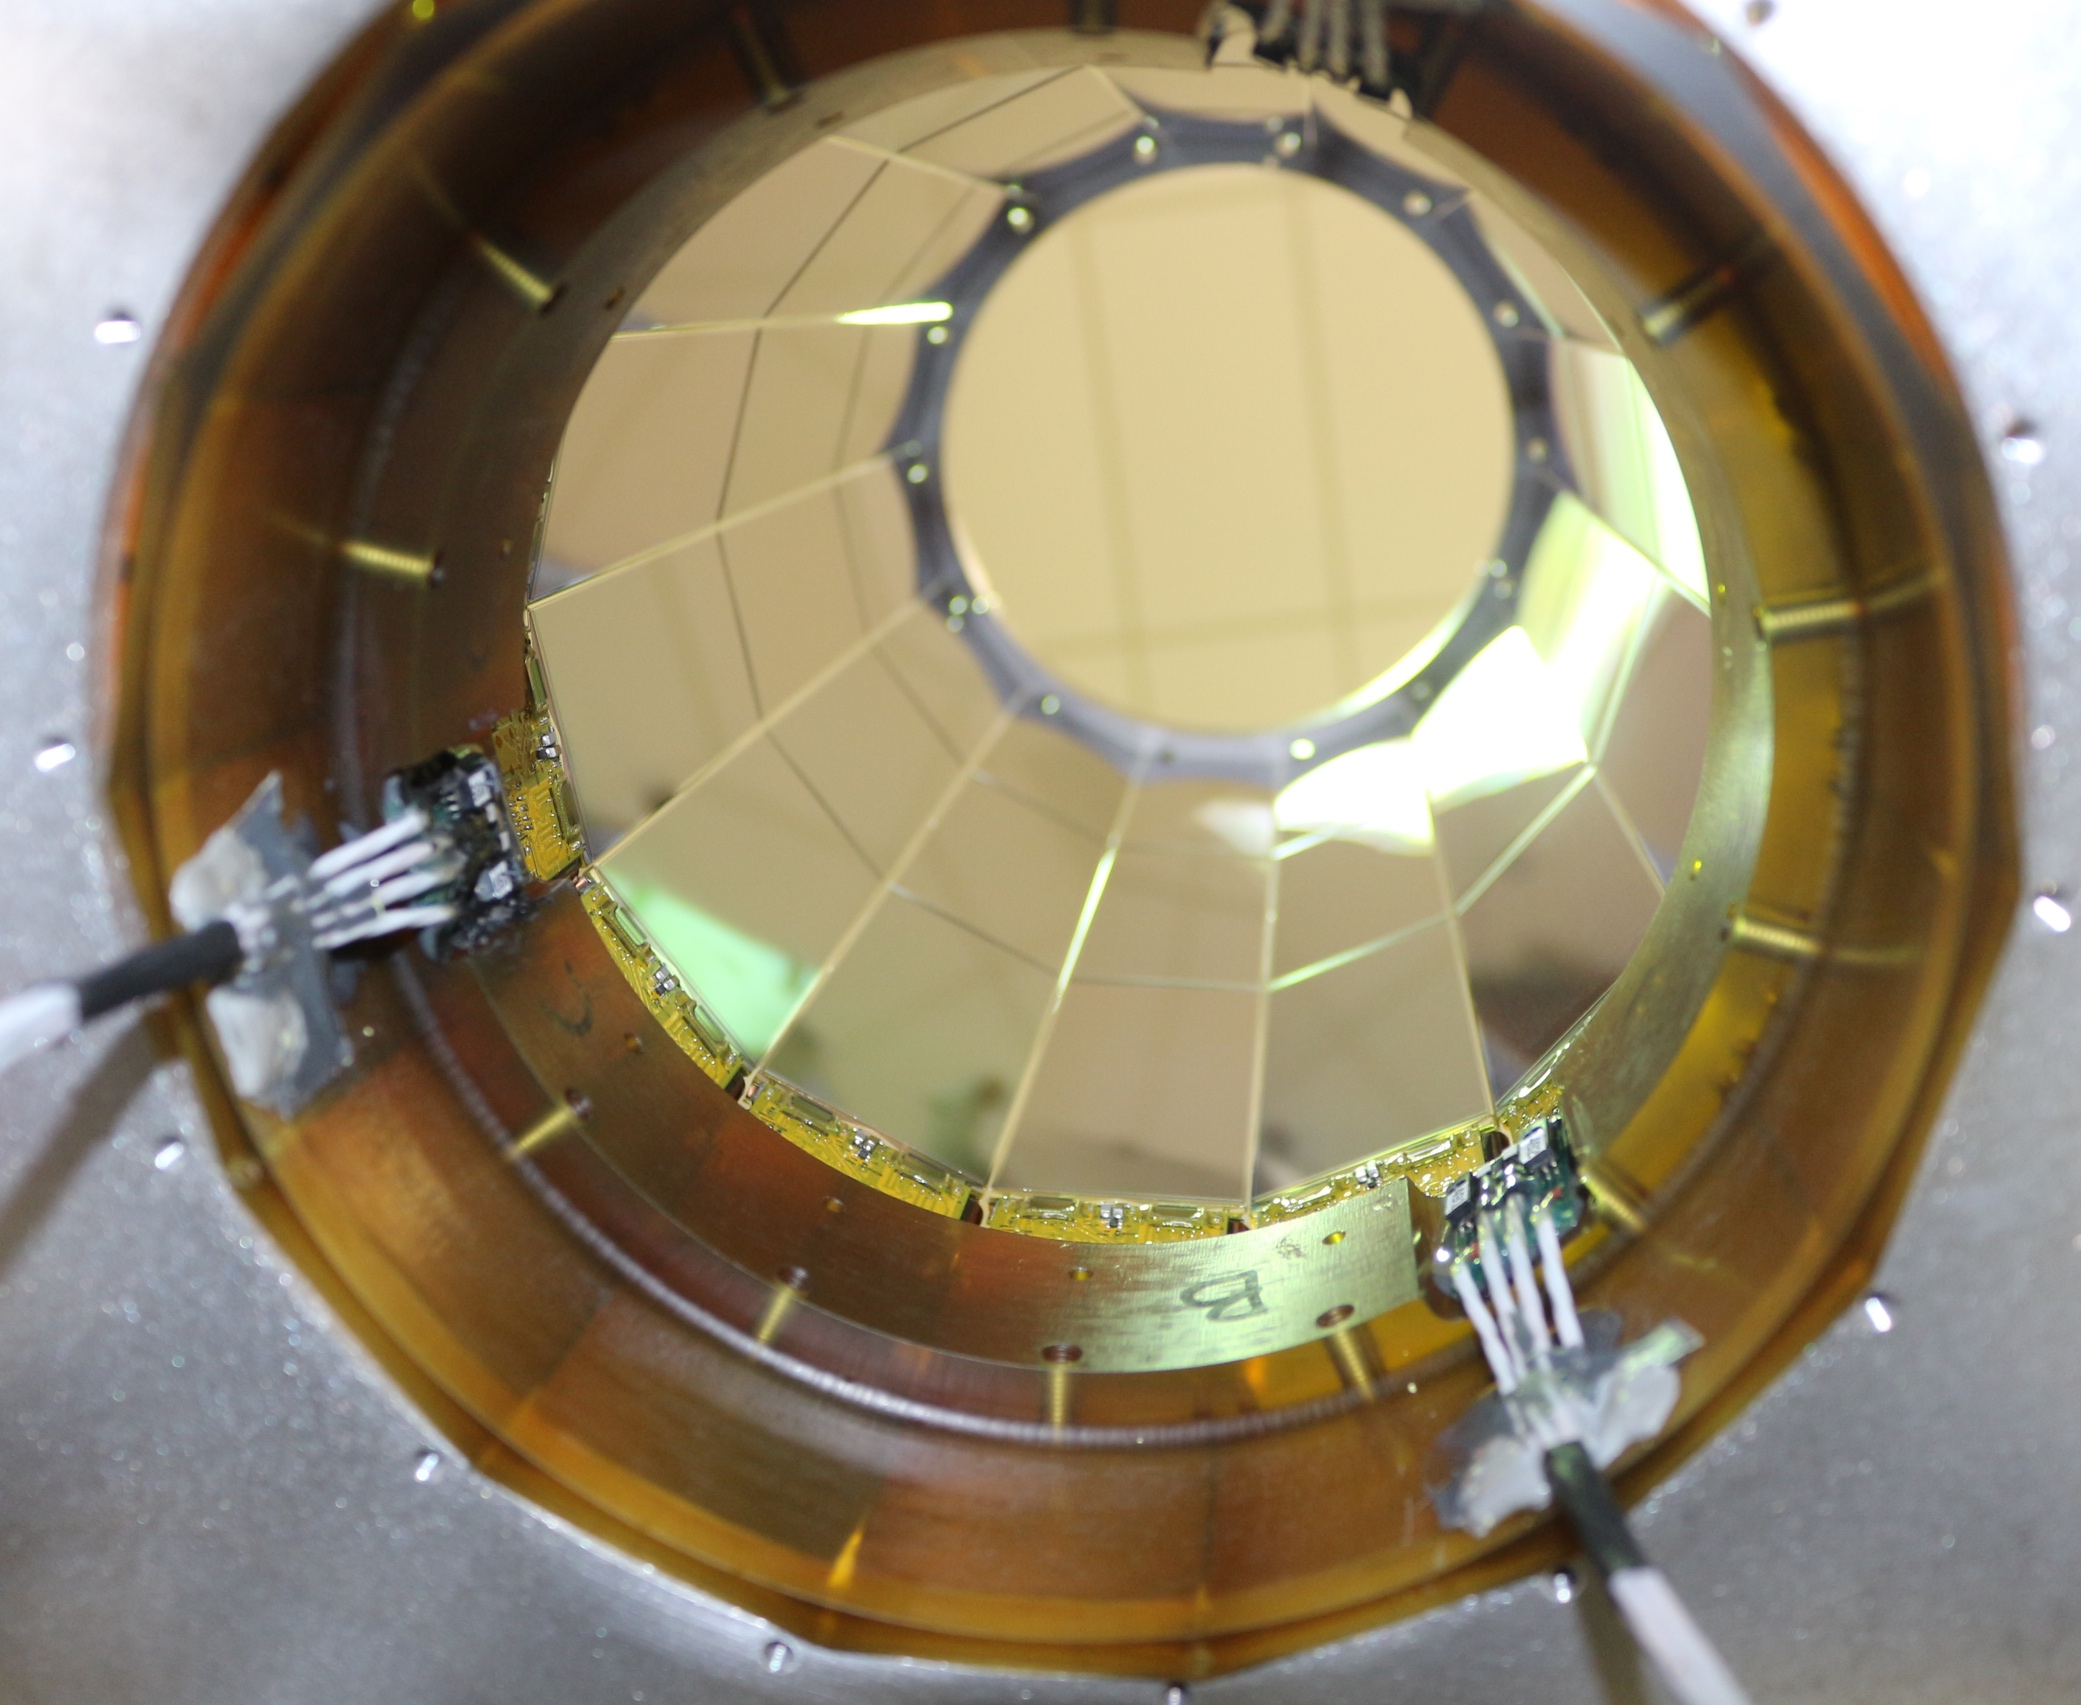
\includegraphics[width=1.0\columnwidth,keepaspectratio]{ambient-sensors.jpg}
\caption{Ambient sensor boards mounted on the upstream rings.}
\label{fig:ambient-sensors}
\end{figure}

Safe operation of the tracker is ensured by Experimental Physics and Industrial Control System (EPICS)-based real-time monitoring of all important operational parameters and status of the hardware components \cite{EPICS}. The software and hardware interlocks continuously monitor the critical system parameters. A multi-level user interface provides safe operation of the SVT by the shift crew and all necessary tools for the system experts (see Fig.~\ref{fig:svt-overview}). Detailed fault charts for the software and hardware monitoring systems were made, and the actions are implemented in the interlock system.

\begin{figure}[hbt] 
\centering 
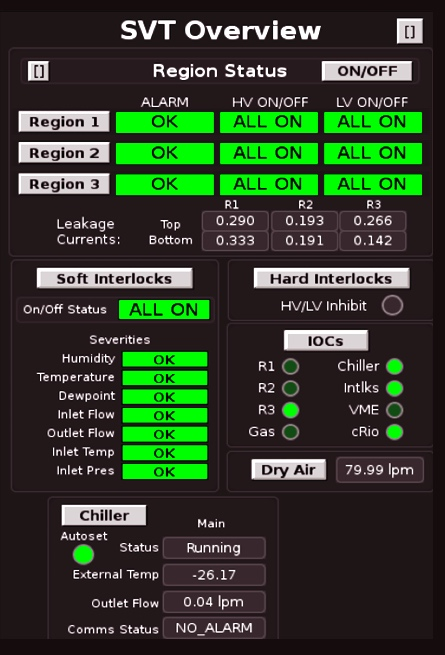
\includegraphics[width=1.0\columnwidth,keepaspectratio]{svt-overview.jpg}
\caption{User interface for the SVT slow controls overview.}
\label{fig:svt-overview}
\end{figure}

The SVT Hardware Interlock System (HIS) is a backup system designed to protect the detector from damage in case the main control system fails or if network communication is lost. This is a standalone system independent from the main EPICS-based slow controls system and does not rely on network communications to safeguard the SVT detector. The HIS is based on the National Instruments CompactRIO (cRIO) Programmable Automation Controller (PAC) platform. The cRIO is a reconfigurable embedded control and acquisition system. The cRIO system's hardware architecture includes I/O modules, a reconfigurable field-programmable gate array (FPGA) chassis, and an embedded controller. The HIS monitors key detector parameters and takes corrective action if a monitored signal is outside of pre-programmed limits. The signals monitored include: HFCB temperature, ambient and detector temperature, humidity, dew point, coolant flow, pressure, temperature, and coolant leak detection (see Fig.~\ref{fig:svt-interlocks}). 

\begin{figure}[hbt] 
\centering 
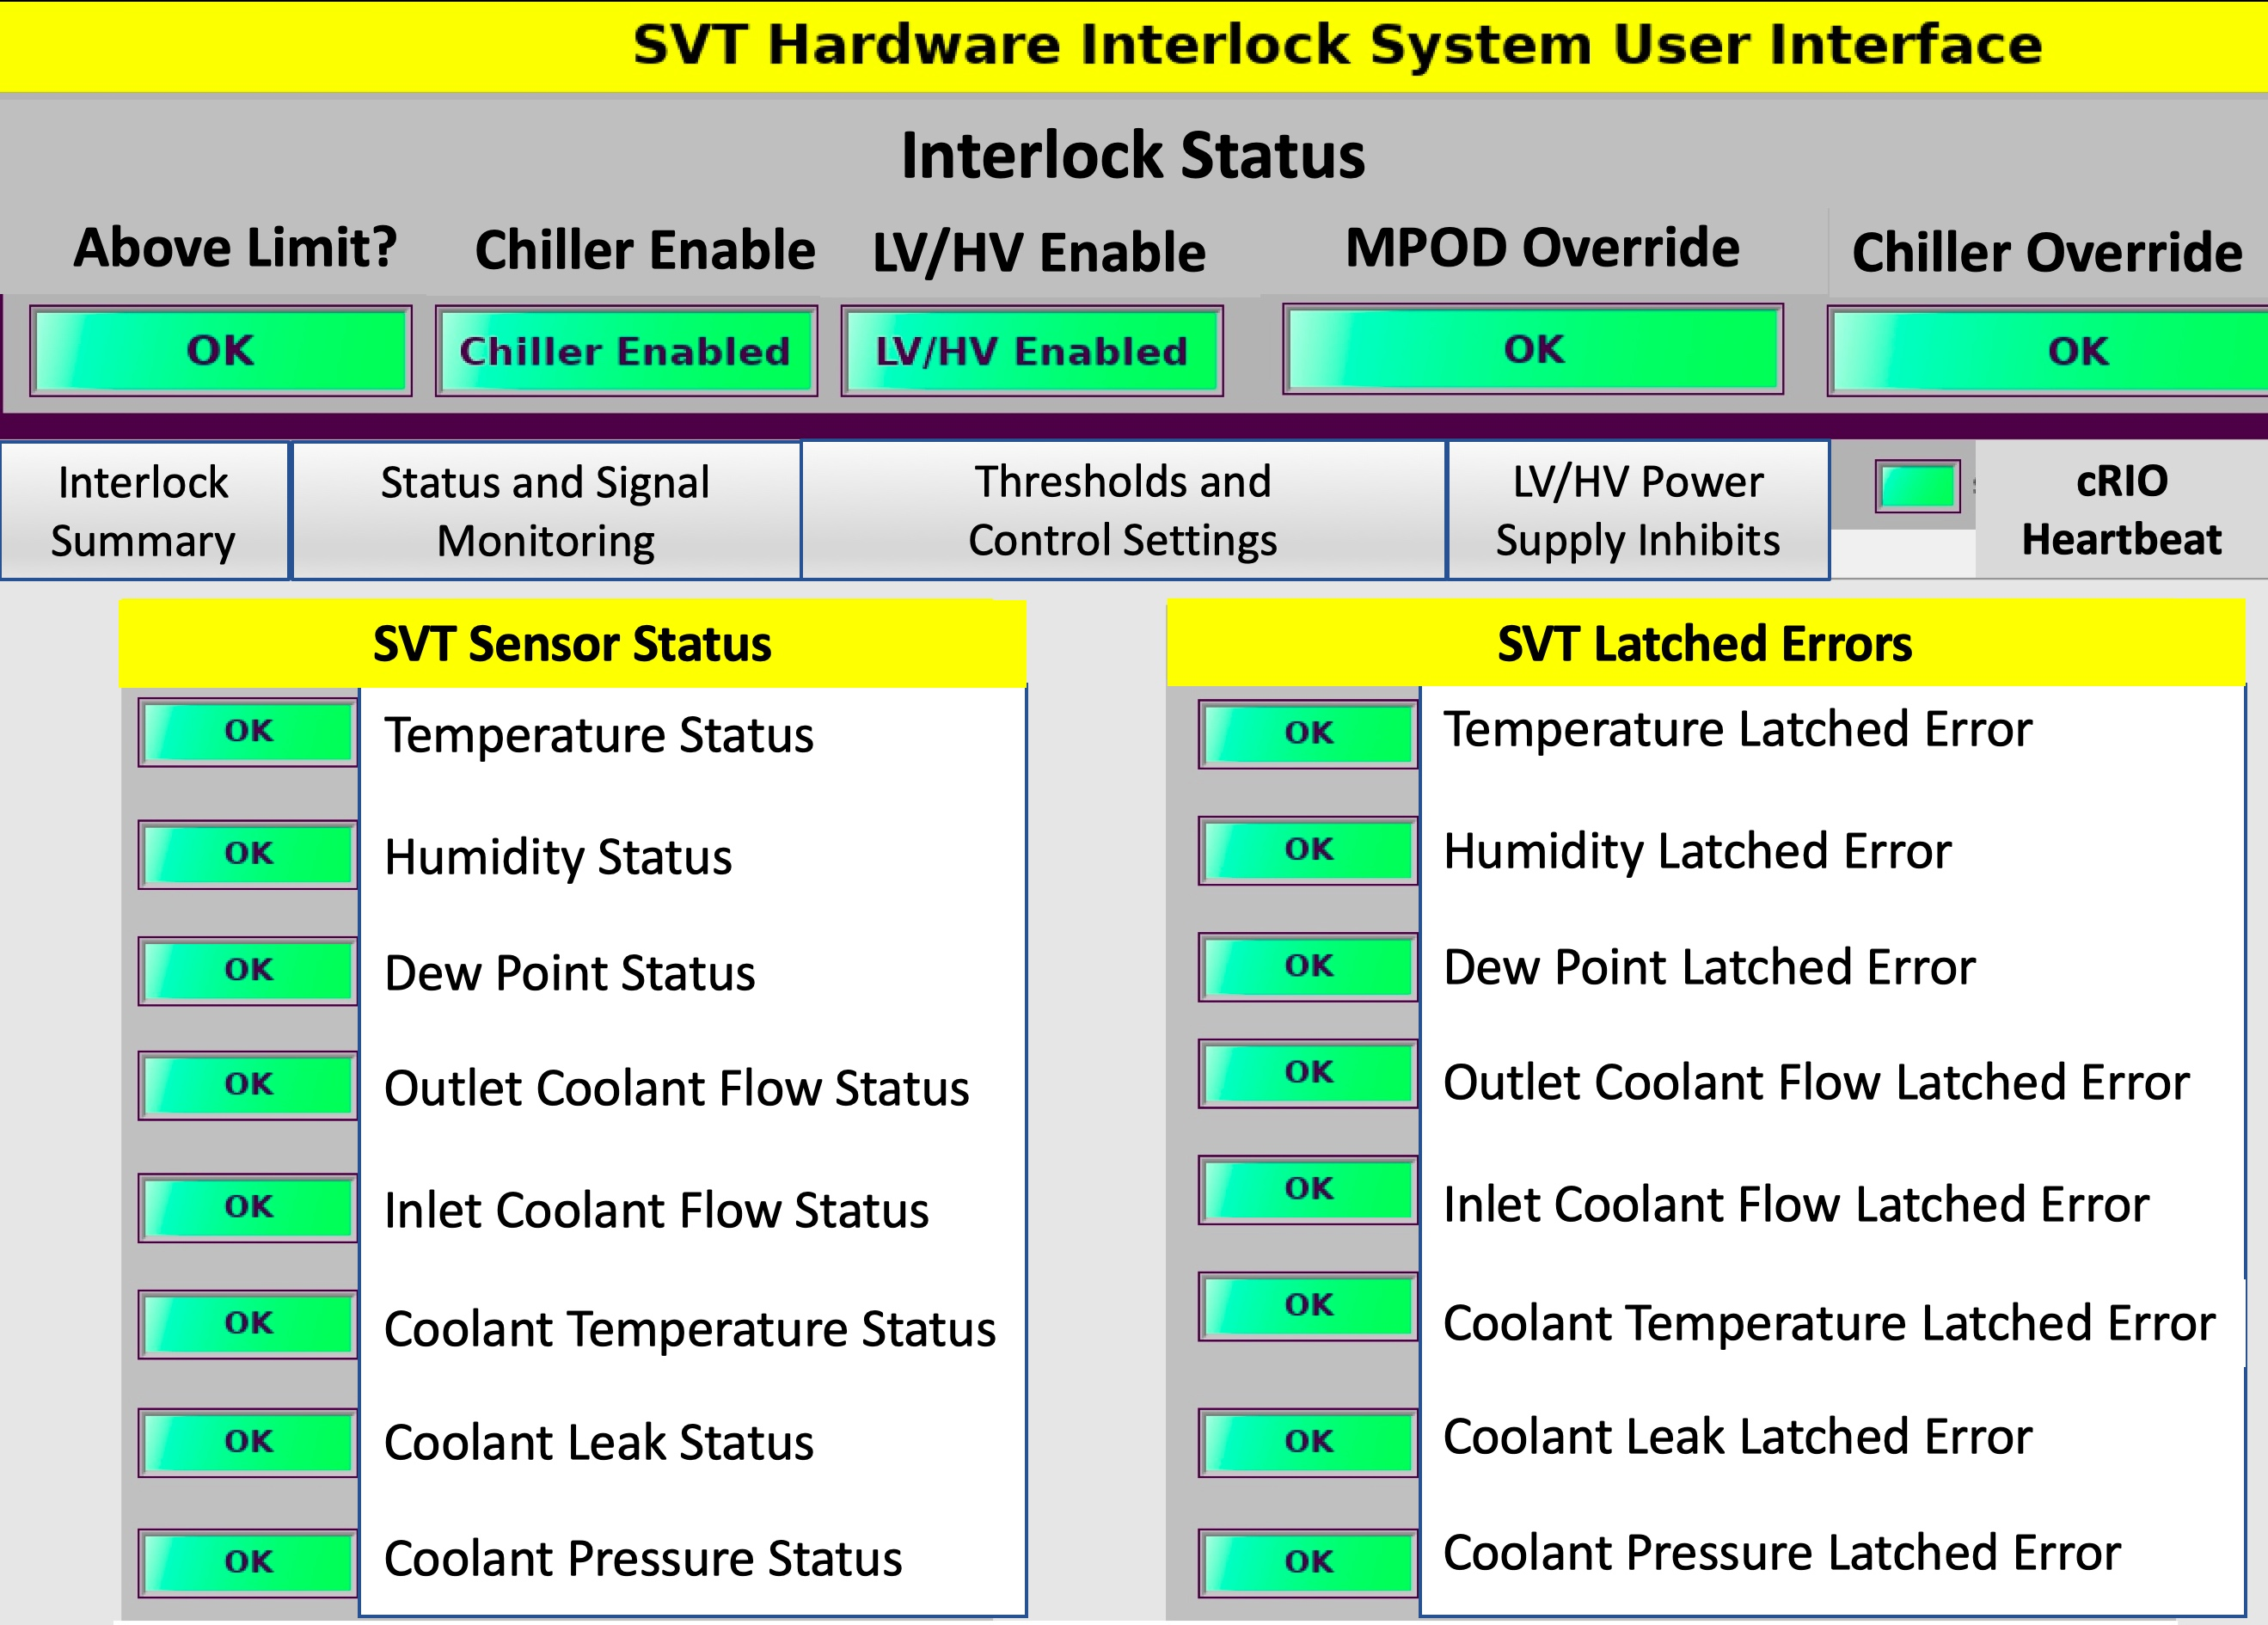
\includegraphics[width=1.0\columnwidth,keepaspectratio]{svt-interlocks.jpg}
\caption{User interface for the SVT hardware interlock system (HIS).}
\label{fig:svt-interlocks}
\end{figure}

Under fault conditions, the hardware interlock system disables the MPOD HV/LV crates via the front panel connector on the MPOD controller. When disabled by the HIS, the EPICS controls are overridden and all channels of the MPOD crate ramp down at their pre-programmed rate. A reset of both the HIS and the EPICS MPOD control is needed in order to re-power the HV and LV channels. Under fault conditions, the HIS shuts off the AC power to the SVT chiller. 

The HIS is the last line of protection for the detector. If the main EPICS slow controls system works correctly, the HIS should never need to take corrective action to protect the detector. The trip levels for the hardware interlock system are slightly out of bounds from the EPICS trip levels to prevent both systems from tripping at the exact same level. The EPICS slow controls system (if working correctly) should always trip before the HIS. The current status of the slow controls and interlocks is reported on the CLAS alarm handler. 

The front panel of the HIS has two interlock keys. These keys allow system experts to update the cRIO system while the SVT detector is powered. These keys are normally locked in the enabled position during detector operation.
The user interface to the HIS allows the operator to remotely monitor the SVT and to set interlock trip levels. The user interface is also used to reset the system after an interlock trip event. 

The performance and stability of the system is tested at various operation temperatures. The observed sensor leakage currents remain below 400 nA in normal operating conditions with coolant at -20$\degree$C. Humidity inside the barrel is kept at $2\%$ by purging dry air. All critical detector operational conditions (currents, voltages, ambient sensor readings, interlocks, etc.) are recorded in a MYA database \cite{MYA} to evaluate system performance and stability. 

\begin{figure}[hbt] 
\centering 
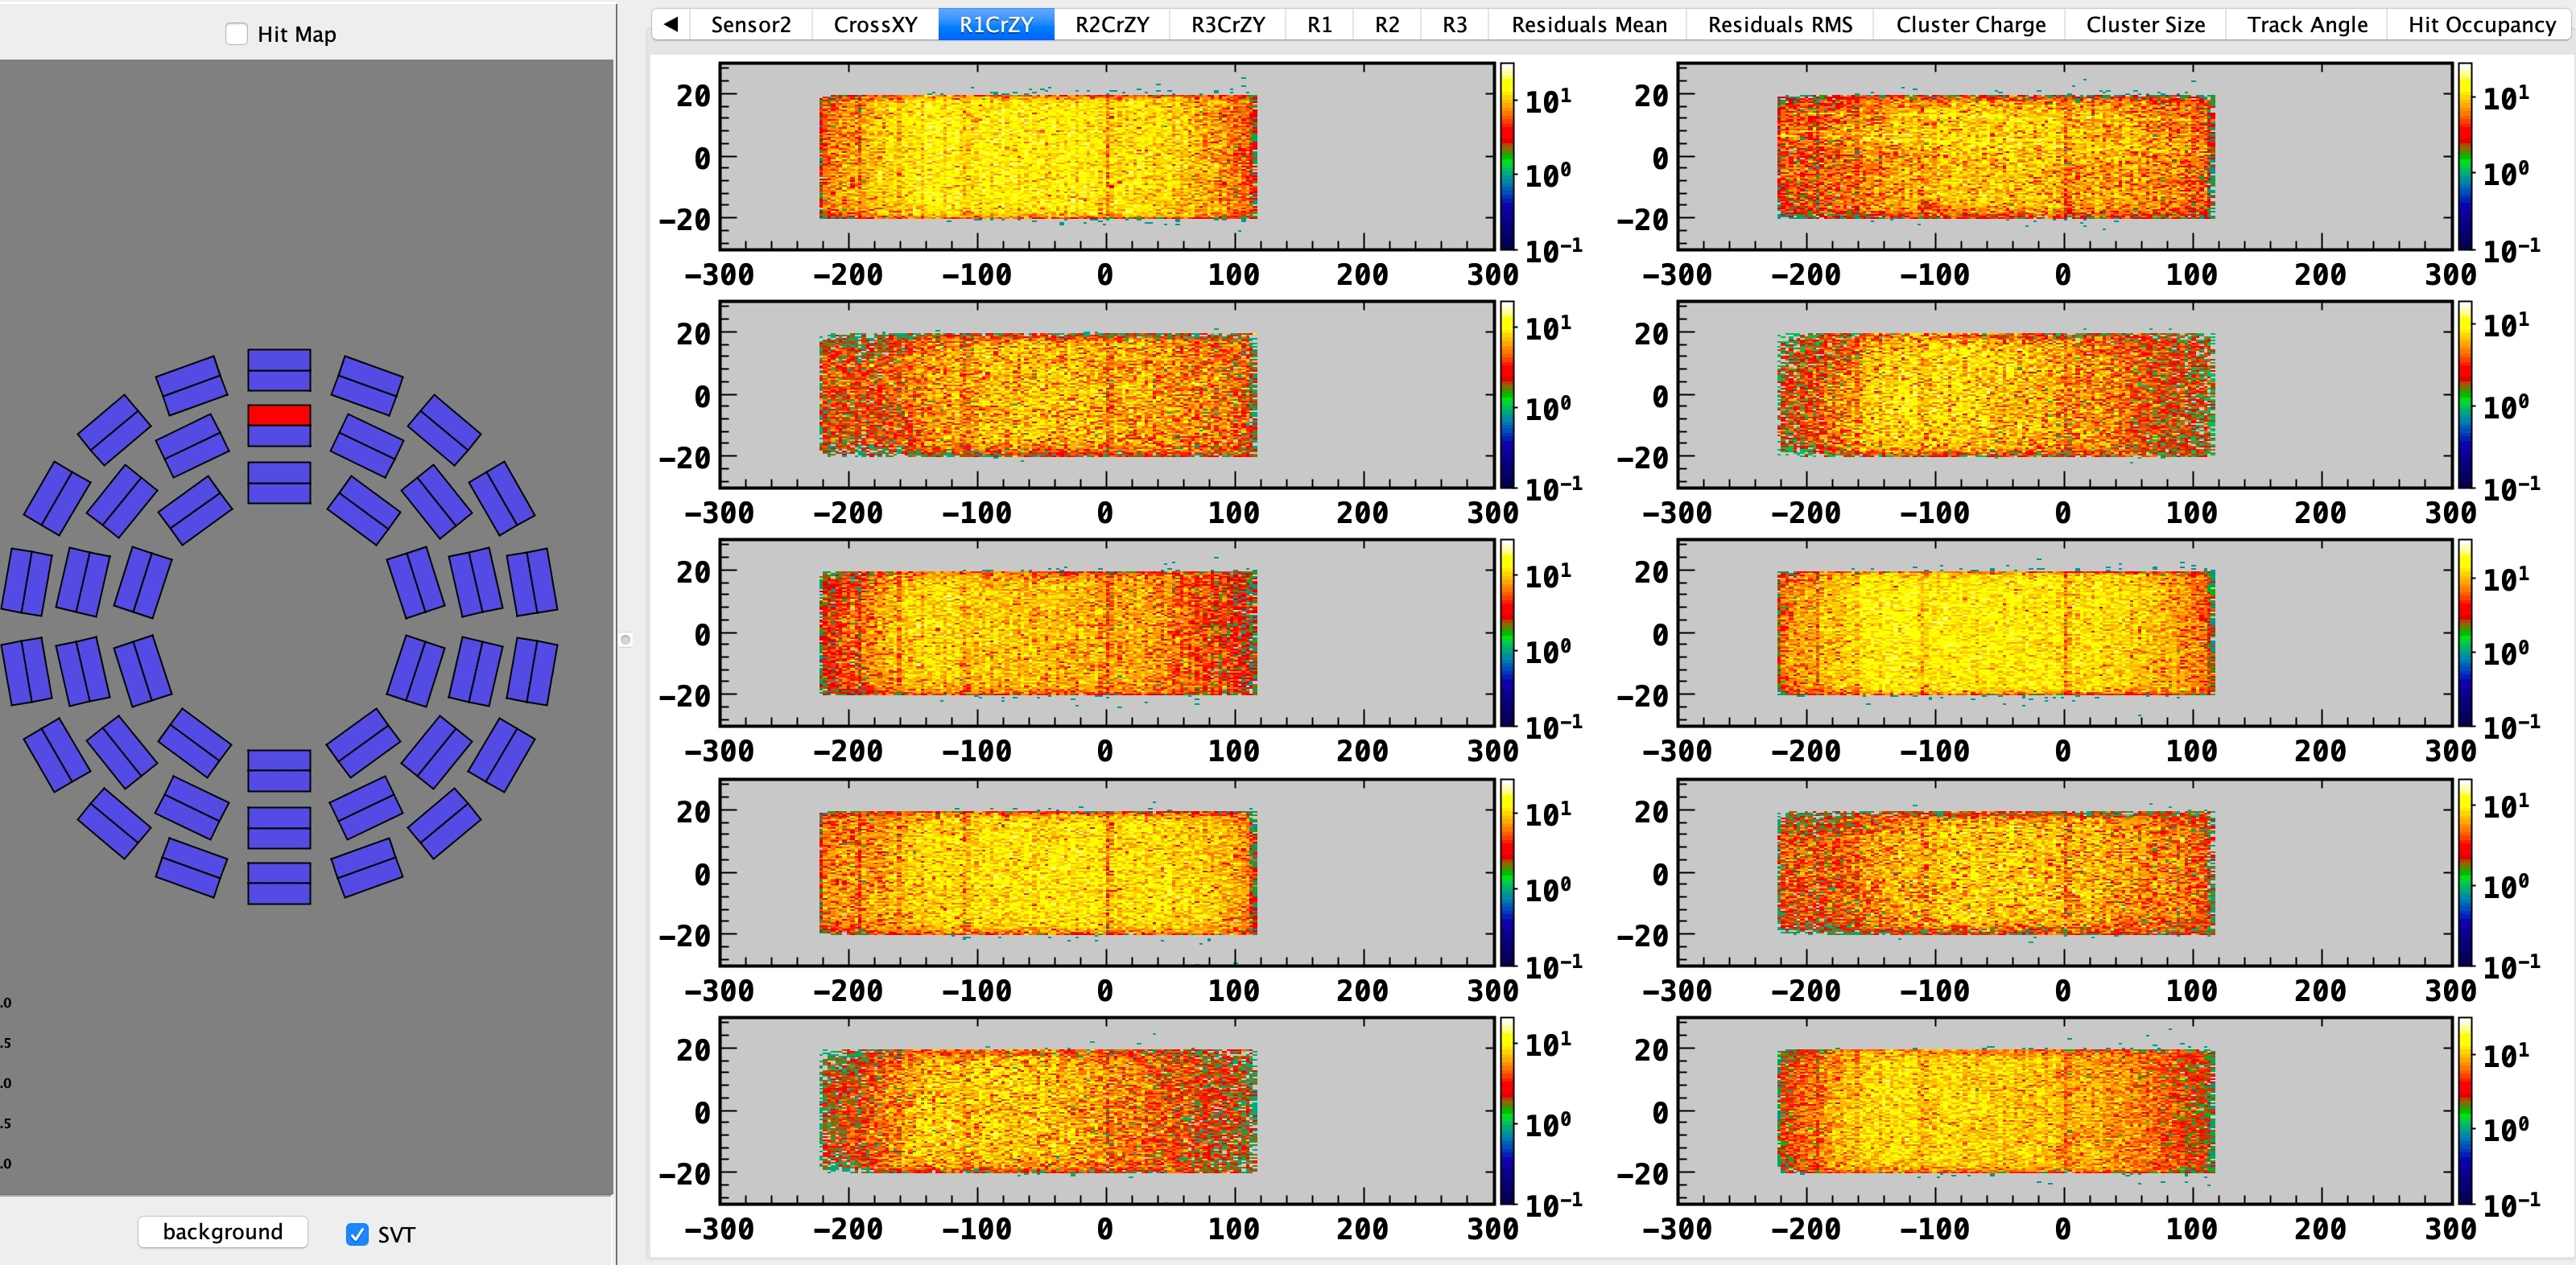
\includegraphics[width=1.0\columnwidth,keepaspectratio]{svt-monitor.jpg}
\caption{SVT detector monitoring interface.}
\label{fig:svt-monitor}
\end{figure}

Java-based data quality monitoring tools were developed to check detector performance both online and offline. The SVT detector monitoring interface is shown in Fig.~\ref{fig:svt-monitor}. The tools allow for checking the status of track reconstruction and performance of the individual modules. Individual sensors can be selected from the SVT layout canvas on the left side of the interface. On the right side a specific set of histograms can be selected with the tabs. The selected tab shows the position of the reconstructed crosses on the surface of the sensors for the first SVT region. The gaps between the sensors are visible.

